\documentclass[fleqn, 11pt]{article}\usepackage[]{graphicx}\usepackage[]{color}
% maxwidth is the original width if it is less than linewidth
% otherwise use linewidth (to make sure the graphics do not exceed the margin)
\makeatletter
\def\maxwidth{ %
  \ifdim\Gin@nat@width>\linewidth
    \linewidth
  \else
    \Gin@nat@width
  \fi
}
\makeatother

\definecolor{fgcolor}{rgb}{0.345, 0.345, 0.345}
\newcommand{\hlnum}[1]{\textcolor[rgb]{0.686,0.059,0.569}{#1}}%
\newcommand{\hlstr}[1]{\textcolor[rgb]{0.192,0.494,0.8}{#1}}%
\newcommand{\hlcom}[1]{\textcolor[rgb]{0.678,0.584,0.686}{\textit{#1}}}%
\newcommand{\hlopt}[1]{\textcolor[rgb]{0,0,0}{#1}}%
\newcommand{\hlstd}[1]{\textcolor[rgb]{0.345,0.345,0.345}{#1}}%
\newcommand{\hlkwa}[1]{\textcolor[rgb]{0.161,0.373,0.58}{\textbf{#1}}}%
\newcommand{\hlkwb}[1]{\textcolor[rgb]{0.69,0.353,0.396}{#1}}%
\newcommand{\hlkwc}[1]{\textcolor[rgb]{0.333,0.667,0.333}{#1}}%
\newcommand{\hlkwd}[1]{\textcolor[rgb]{0.737,0.353,0.396}{\textbf{#1}}}%
\let\hlipl\hlkwb

\usepackage{framed}
\makeatletter
\newenvironment{kframe}{%
 \def\at@end@of@kframe{}%
 \ifinner\ifhmode%
  \def\at@end@of@kframe{\end{minipage}}%
  \begin{minipage}{\columnwidth}%
 \fi\fi%
 \def\FrameCommand##1{\hskip\@totalleftmargin \hskip-\fboxsep
 \colorbox{shadecolor}{##1}\hskip-\fboxsep
     % There is no \\@totalrightmargin, so:
     \hskip-\linewidth \hskip-\@totalleftmargin \hskip\columnwidth}%
 \MakeFramed {\advance\hsize-\width
   \@totalleftmargin\z@ \linewidth\hsize
   \@setminipage}}%
 {\par\unskip\endMakeFramed%
 \at@end@of@kframe}
\makeatother

\definecolor{shadecolor}{rgb}{.97, .97, .97}
\definecolor{messagecolor}{rgb}{0, 0, 0}
\definecolor{warningcolor}{rgb}{1, 0, 1}
\definecolor{errorcolor}{rgb}{1, 0, 0}
\newenvironment{knitrout}{}{} % an empty environment to be redefined in TeX

\usepackage{alltt}
\usepackage{amsmath}
\usepackage{amssymb}
\usepackage{geometry}
\usepackage{graphicx}
\usepackage{bm}
\usepackage{url}
\usepackage{hyperref}
\usepackage{enumerate}
\usepackage{fullpage}
\IfFileExists{upquote.sty}{\usepackage{upquote}}{}
\begin{document}

\setlength\parindent{0pt}

\begin{center}
\textbf{Lecture 11: Inference for One Proportion}\\
\textbf{STAT 630, Fall 2021}\\
\hrulefill
\end{center}

\textbf{Bernoulli random variables and properties of the sample proportion}\\

Let $X$ be a binary random variable following a \textbf{Bernoulli distribution} with probability $p$.  We can write this as $X \sim \text{Bern}(p)$.  Find the probability mass function, expectation, and variance of~$X$.\\  
% \vspace{8cm}

{\color{blue}Probability mass function:}
\begin{table}[ht]
{\color{blue}
\begin{tabular}{l|l|l}
$x$ & 0 & 1\\
\hline
$P(X=x)$ & $1-p$ & $p$
\end{tabular}}
\end{table}

{\color{blue}
\begin{align*}
E(X) &= \sum_{x} x \cdot P(X=x) = 0 \cdot (1-p) + 1 \cdot p = p
\end{align*}

\begin{align*}
Var(X) &= \sum_{x} (x - E(X))^2 \cdot P(X=x) = (0-p)^2 (1-p) + (1-p)^2 p\\
&= p^2 (1-p) + (1-p)^2 p = p(1-p) \cdot [p + (1-p)] = p(1-p)\\
\end{align*}
}


Let $X_1, X_2, \cdots, X_n$ be independent random variables (i.e., a random sample) from Bern($p$).  For example, the parameter $p$ is the \textbf{population proportion} of individuals that support a certain political candidate; $X_i=1$ if the $i$-th randomly sampled person votes for the candidate, and $X_i=0$ otherwise.  We can estimate the population proportion with the \textbf{sample proportion} defined as:
\begin{align*}
\hat{p} = \frac{1}{n} \sum_{i=1}^n X_i
\end{align*}
Find the expectation and variance of the sample proportion:\\
{\color{blue}
\begin{align*}
E(\hat{p}) & = E\left( \frac{1}{n} \sum_{i=1}^n X_i \right) = \frac{1}{n} \sum_{i=1}^n E(X_i) = \frac{np}{n} = p\\
Var(\hat{p}) &= Var \left( \frac{1}{n} \sum_{i=1}^n X_i \right) = \frac{1}{n^2} \sum_{i=1}^n Var(X_i) = \frac{np(1-p)}{n^2} = \frac{p(1-p)}{n}
\end{align*}}
\clearpage

\textbf{Central limit theorem for sample proportion}\\

Since the sample proportion $\hat{p} = \frac{1}{n} \sum_{i=1}^n X_i$ is the sample mean of Bernoulli random variables, the central limit theorem gives the following approximation for the sampling distribution of $\hat{p}$:  
\begin{align*}
\hat{p} \sim N\left(p, \sqrt{\frac{p(1-p)}{n}} \right)
\end{align*}
The approximation should only be used if $np \geq 10$ and $n(1-p) \geq 10$.  This is often called the ``success-failure'' condition.\\

\textbf{Remark}:  Let $Y = n\hat{p} = \sum_{i=1}^n X_i$, which is the sum of independent Bernoulli random variables.  Then the exact distribution $Y$ follows is a binomial distribution with parameters $n$ and $p$.  However, as long as the conditions are satisfied, it is often easier to use the normal approximation.\\
\vspace{22pt}

\textbf{1-$\alpha$ confidence interval for population proportion p}
\begin{align*}
\hat{p} \pm z_{\alpha / 2}  \sqrt{\frac{\hat{p}(1-\hat{p})}{n}}
\end{align*}
Conditions: $n \hat{p} \geq 10$ and $n (1-\hat{p}) \geq 10$, and the sample observations are independent.  Generally, the independence condition is satisfied if the data come from a simple random sample.\\
\vspace{11pt}

\textbf{Derivation}:\\
By the central limit theorem, $Z = \frac{\hat{p} - p}{\sqrt{p(1-p)/n}} \sim N(0,1)$ approximately.  Therefore,
\begin{align*}
P \left(-z_{\alpha/2} < \frac{\hat{p} - p}{\sqrt{p(1-p)/n}} < z_{\alpha/2} \right) = 1-\alpha
\end{align*}
After rearranging terms:
\begin{align*}
P \left(\hat{p} - z_{\alpha/2}\sqrt{p(1-p)/n} < p < \hat{p} + z_{\alpha/2}\sqrt{p(1-p)/n} \right) = 1-\alpha
\end{align*}
The issue with this interval is the endpoints are in terms of the unknown population proportion parameter $p$.  As an approximation, we replace $\sqrt{p(1-p)/n}$ with $\sqrt{\hat{p}(1-\hat{p})/n}$ when calculating the interval.\\
\clearpage

\textbf{Sample size determination}\\
Determine the sample size needed so that the confidence interval will have a margin of error $\pm E$ with confidence level $1-\alpha$.
% \vspace{8cm}
{\color{blue}
\begin{align*}
E = z_{\alpha/2} \sqrt{\frac{\hat{p}(1-\hat{p})}{n}}
\implies E^2 = z^2_{\alpha/2} \frac{\hat{p}(1-\hat{p})}{n} \implies n = \frac{z^2_{\alpha/2} \hat{p}(1-\hat{p})}{E^2}\\
\end{align*}

If no data has been collected, $\hat{p}=0.5$ gives the largest sample size.  Why?\\
Let $f(p) = p(1-p) = -p^2 + p$. Then $f'(p) = -2p + 1$; setting $f'(p)=0$ gives $p=1/2$ as the maximum.  This can be checked graphically as well since $f(p) = -p^2 + p$ is a parabola facing down.
}
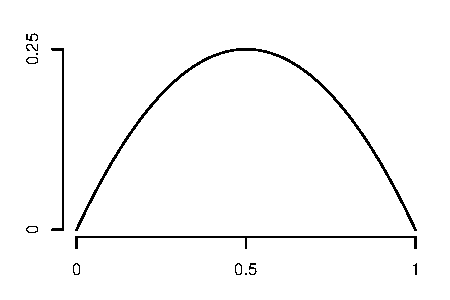
\includegraphics[scale=0.65]{parabola.pdf}


\textbf{Ex1}:  At a survey poll before the elections, candidate A receives the support of 650 voters in a random sample of 1200 voters.  
\begin{enumerate}[(a)]
\item Construct a 95\% confidence interval for the population proportion $p$ of voters that support candidate A.  Check the conditions for the interval.
\item Find the sample size needed so that the margin of error will be $\pm 0.01$ with confidence level 0.95.
\end{enumerate}
{\color{blue}
\emph{Solution}:\\
(a) The conditions for the interval are satisfied since $n\hat{p} = 650 \geq 10$ and $n(1-\hat{p}) = 550 \geq 10$, and the voters were random sampled.\\

The sample proportion is $\hat{p} = 650/1200 = 0.54$ and $n=1200$.
\begin{align*}
0.54 \pm 1.96 \sqrt{\frac{(0.54)(0.46)}{1200}} \implies (0.512, 0.568)
\end{align*}
We are 95\% confident that the population proportion of voters that support candidate A is between 0.512 and 0.568.\\

(b) Using $\hat{p} = 0.5$ to get the largest sample size:
\begin{align*}
n = \frac{1.96^2 (0.5)(1-0.5)}{(0.01)^2} = 9604\\
\end{align*}
}
\newpage

\textbf{Hypothesis test for population proportion p}\\

Null and alternative hypotheses:\\
$H_0$: $p = p_0$\\
$H_A$: $p > p_0$ or $p < p_0$ or $p \neq p_0$\\

Test statistic:  Assuming $H_0$ is true, $\hat{p} \sim N(p_0, \sqrt{p_0 (1-p_0)/n})$.  Standardize to get the following $z$-test statistic:
\begin{align*}
z = \frac{\hat{p} - p_0}{\sqrt{p_0 (1-p_0)/n}}
\end{align*}

Once the z-test statistic is computed, the $p$-value can be computed to decide whether to reject or not reject the null hypothesis.\\

Conditions: $n p_0 \geq 10$ and $n (1-p_0) \geq 10$, and independence.\\
\vspace{11pt}

\textbf{Ex2}: A simple random sample of 1,028 US adults in March 2013 found that 56\% support nuclear arms reduction.  Does this provide convincing evidence that a majority of Americans support nuclear arms reduction?\footnote{\url{https://news.gallup.com/poll/161198/favor-russian-nuclear-arms-reductions.aspx}}\\ 

{\color{blue}The conditions for the test are satisfied since $n p_0 = n (1-p_0) = 1028(0.5) \geq 10$, and the respondents were randomly sampled.\\

$H_0: p = 0.5$\\
$H_A: p > 0.5$\\

The sample proportion is $\hat{p} = 0.56$ and $n=1028$.\\

Test statistic:
\begin{align*}
z = \frac{0.56 - 0.5}{\sqrt{\frac{0.5(1-0.5)}{1028}}} = 3.85
\end{align*}

$p$-value $=P(Z > 3.85) = \texttt{1 - pnorm(3.85)} \approx 0$\\

Since the $p$-value $\approx 0$, we reject $H_0$.  The poll provides convincing evidence that a majority of Americans support nuclear arms reduction.}

\newpage

\textbf{Simulation Study}:  Simulating the sampling distribution of the sample proportion when:
\begin{itemize}
\item the population size is 1 million
\item the sample size is $n=1000$
\item the population proportion is $p=0.6$
\end{itemize}

\begin{knitrout}
\definecolor{shadecolor}{rgb}{0.969, 0.969, 0.969}\color{fgcolor}\begin{kframe}
\begin{alltt}
\hlkwd{set.seed}\hlstd{(}\hlnum{999}\hlstd{)}
\hlstd{pop_size} \hlkwb{<-} \hlnum{10}\hlopt{^}\hlnum{6}
\hlstd{n} \hlkwb{<-} \hlnum{1000}
\hlstd{population} \hlkwb{<-} \hlkwd{c}\hlstd{(}\hlkwd{rep}\hlstd{(}\hlnum{0}\hlstd{,} \hlnum{0.4}\hlopt{*}\hlstd{pop_size),} \hlkwd{rep}\hlstd{(}\hlnum{1}\hlstd{,} \hlnum{0.6}\hlopt{*}\hlstd{pop_size))}
\hlstd{phats} \hlkwb{<-} \hlkwd{c}\hlstd{()} \hlcom{# initialize vector for sample proportions}
\hlkwa{for}\hlstd{(i} \hlkwa{in} \hlnum{1}\hlopt{:}\hlnum{5000}\hlstd{) \{}
  \hlstd{samp} \hlkwb{<-} \hlkwd{sample}\hlstd{(population,} \hlkwc{size} \hlstd{= n)}
  \hlstd{phats[i]} \hlkwb{<-} \hlkwd{sum}\hlstd{(samp)} \hlopt{/} \hlstd{n}
\hlstd{\}}
\end{alltt}
\end{kframe}
\end{knitrout}
\begin{knitrout}
\definecolor{shadecolor}{rgb}{0.969, 0.969, 0.969}\color{fgcolor}\begin{kframe}
\begin{alltt}
\hlkwd{par}\hlstd{(}\hlkwc{mfrow} \hlstd{=} \hlkwd{c}\hlstd{(}\hlnum{1}\hlstd{,} \hlnum{2}\hlstd{),} \hlkwc{cex}\hlstd{=}\hlnum{0.8}\hlstd{)}
\hlkwd{hist}\hlstd{(phats,} \hlkwc{xlab} \hlstd{=} \hlstr{"Sample Proportions"}\hlstd{,} \hlkwc{main} \hlstd{=} \hlstr{""}\hlstd{)}
\hlkwd{abline}\hlstd{(}\hlkwc{v} \hlstd{=} \hlnum{0.6}\hlstd{,} \hlkwc{col} \hlstd{=} \hlstr{"red"}\hlstd{,} \hlkwc{lwd} \hlstd{=} \hlnum{2}\hlstd{)}
\hlkwd{qqnorm}\hlstd{(phats)}
\hlkwd{qqline}\hlstd{(phats)}
\end{alltt}
\end{kframe}
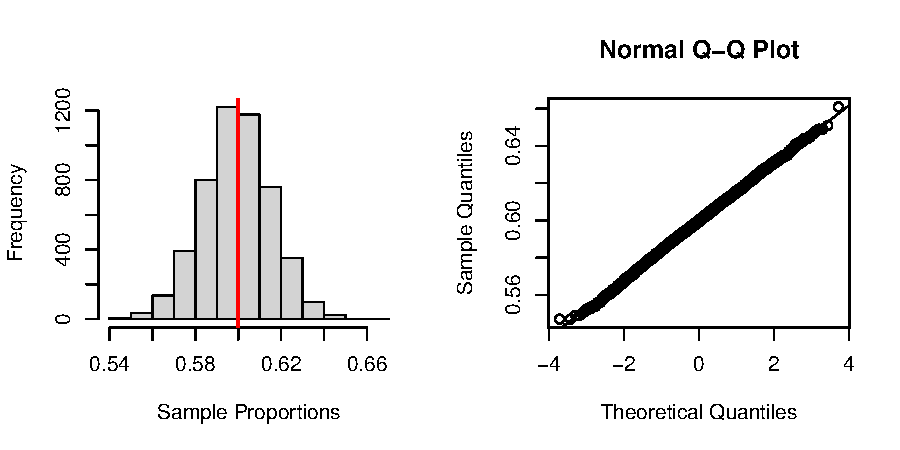
\includegraphics[width=\maxwidth]{figure/unnamed-chunk-2-1} 
\end{knitrout}

\begin{knitrout}
\definecolor{shadecolor}{rgb}{0.969, 0.969, 0.969}\color{fgcolor}\begin{kframe}
\begin{alltt}
\hlkwd{sd}\hlstd{(phats)}
\end{alltt}
\begin{verbatim}
## [1] 0.01578796
\end{verbatim}
\begin{alltt}
\hlkwd{sqrt}\hlstd{(}\hlnum{0.6} \hlopt{*} \hlnum{0.4} \hlopt{/} \hlnum{1000}\hlstd{)}
\end{alltt}
\begin{verbatim}
## [1] 0.01549193
\end{verbatim}
\end{kframe}
\end{knitrout}



\end{document}




